\chapter{Sistema proposto}
\label{cap:sistema_proposto}

% Geladeiras inteligentes existentes
    % Funcionalidades


Geladeiras inteligentes têm sido lançadas por fabricantes como Samsung e LG, tendo estas muitas características em comum. Em relação ao modelo tradicional, essas geladeiras trazem uma maior interação dos usuários a partir de uma interface \textit{touch screen}, além do uso de câmeras no interior do equipamento.

A partir da interface é possível criar lembretes para os demais moradores da casa, ler notícias e ver a previsão do tempo. Além disso, é possível adicionar itens ao calendário e visualizar receitas. Por outro lado, conta-se com o auxílio de assistentes virtuais como a Alexa, da Amazon, e a Cortana da Microsoft, que possibilitam que ações sejam executadas a partir de comandos de voz como, por exemplo, compras de novos produtos. 

Apesar de as funcionalidades serem úteis e interessantes, geladeiras como estas não se atentaram à observação dos hábitos e preferências por produtos de seus usuários. Como exemplo, tais eletrodomésticos não são capazes de inferir que um usuário seja vegetariano ou que tenha intolerância à lactose.

    
% Componentes do sistema (geladeira, aplicação, servidor, mercado) que estão dispostos na arquitetura proposta,

% Onde o trabalho atua especificamente
    % O que vai adicionar
    % Quais as funcionalidades

O sistema proposto nesse capítulo foca na questão mencionada e apresenta um modelo de geladeira inteligente que seja capaz de observar os hábitos de seus usuários e disponibilizar uma experiência personalizada de modo a facilitar o seu dia a dia. Para tanto, criou-se uma modelagem que engloba os diversos componentes do sistema além da geladeira em si. Desse modo, o sistema foi dividido em três elementos globais: a geladeira, servidor e mercado.

O primeiro deles, a geladeira, contém dois subsistemas, um mecanismo de leitura de itens contidos e a interface. Já o servidor contém bases de dados e processos que compõe o sistema de análise de interações e recomendação. E, por fim, o mercado é responsável por permitir a compra de produtos, a verificação de disponibilidade destes e a obtenção de informações detalhadas sobre.
    
Baseando-se nos três componentes, o sistema proposto disponibiliza, como funcionalidades, a listagem dos produtos contidos, compras automáticas, produtos com expiração de validade iminente e recomendação de produtos e receitas, como será detalhado posteriormente.
    
    
%\section{Arquitetura}
%####################################################%
O modelo criado foi subdividido em duas modelagens, sendo elas, lógica e física. A primeira apresenta os componentes do sistema abstraindo as tecnologias envolvidas na sua composição, focando, desse modo, nas funcionalidades. Já o modelo físico complementa a visão lógica a partir do detalhamento de cada componente bem como as tecnologias empregadas em suas respectivas implementações.

\section{Modelo lógico}

O modelo lógico do sistema proposto neste trabalho é apresentado na Figura \ref{fig:c4_modelo_logico}. Pode-se observar, portanto, cinco camadas: aplicação, serviços, repositórios, processamento e agente externo. A primeira delas, de aplicação, envolve os componentes externos ao servidor principal, mas que são relacionados ao sistema, sendo eles, geladeira e interface de usuário. Já as demais camadas, de serviços, repositórios e processamento, se encontram dentro do servidor%, sendo estas separadas por módulos
. Por fim, a camada de agente externo abriga o mercado ao qual apresenta um funcionamento independente à arquitetura aqui proposta.

% Figura

% Explicar figura
% Explicação das camadas
\begin{figure}[htb]
    \caption{Modelo lógico}
    \label{fig:c4_modelo_logico}
    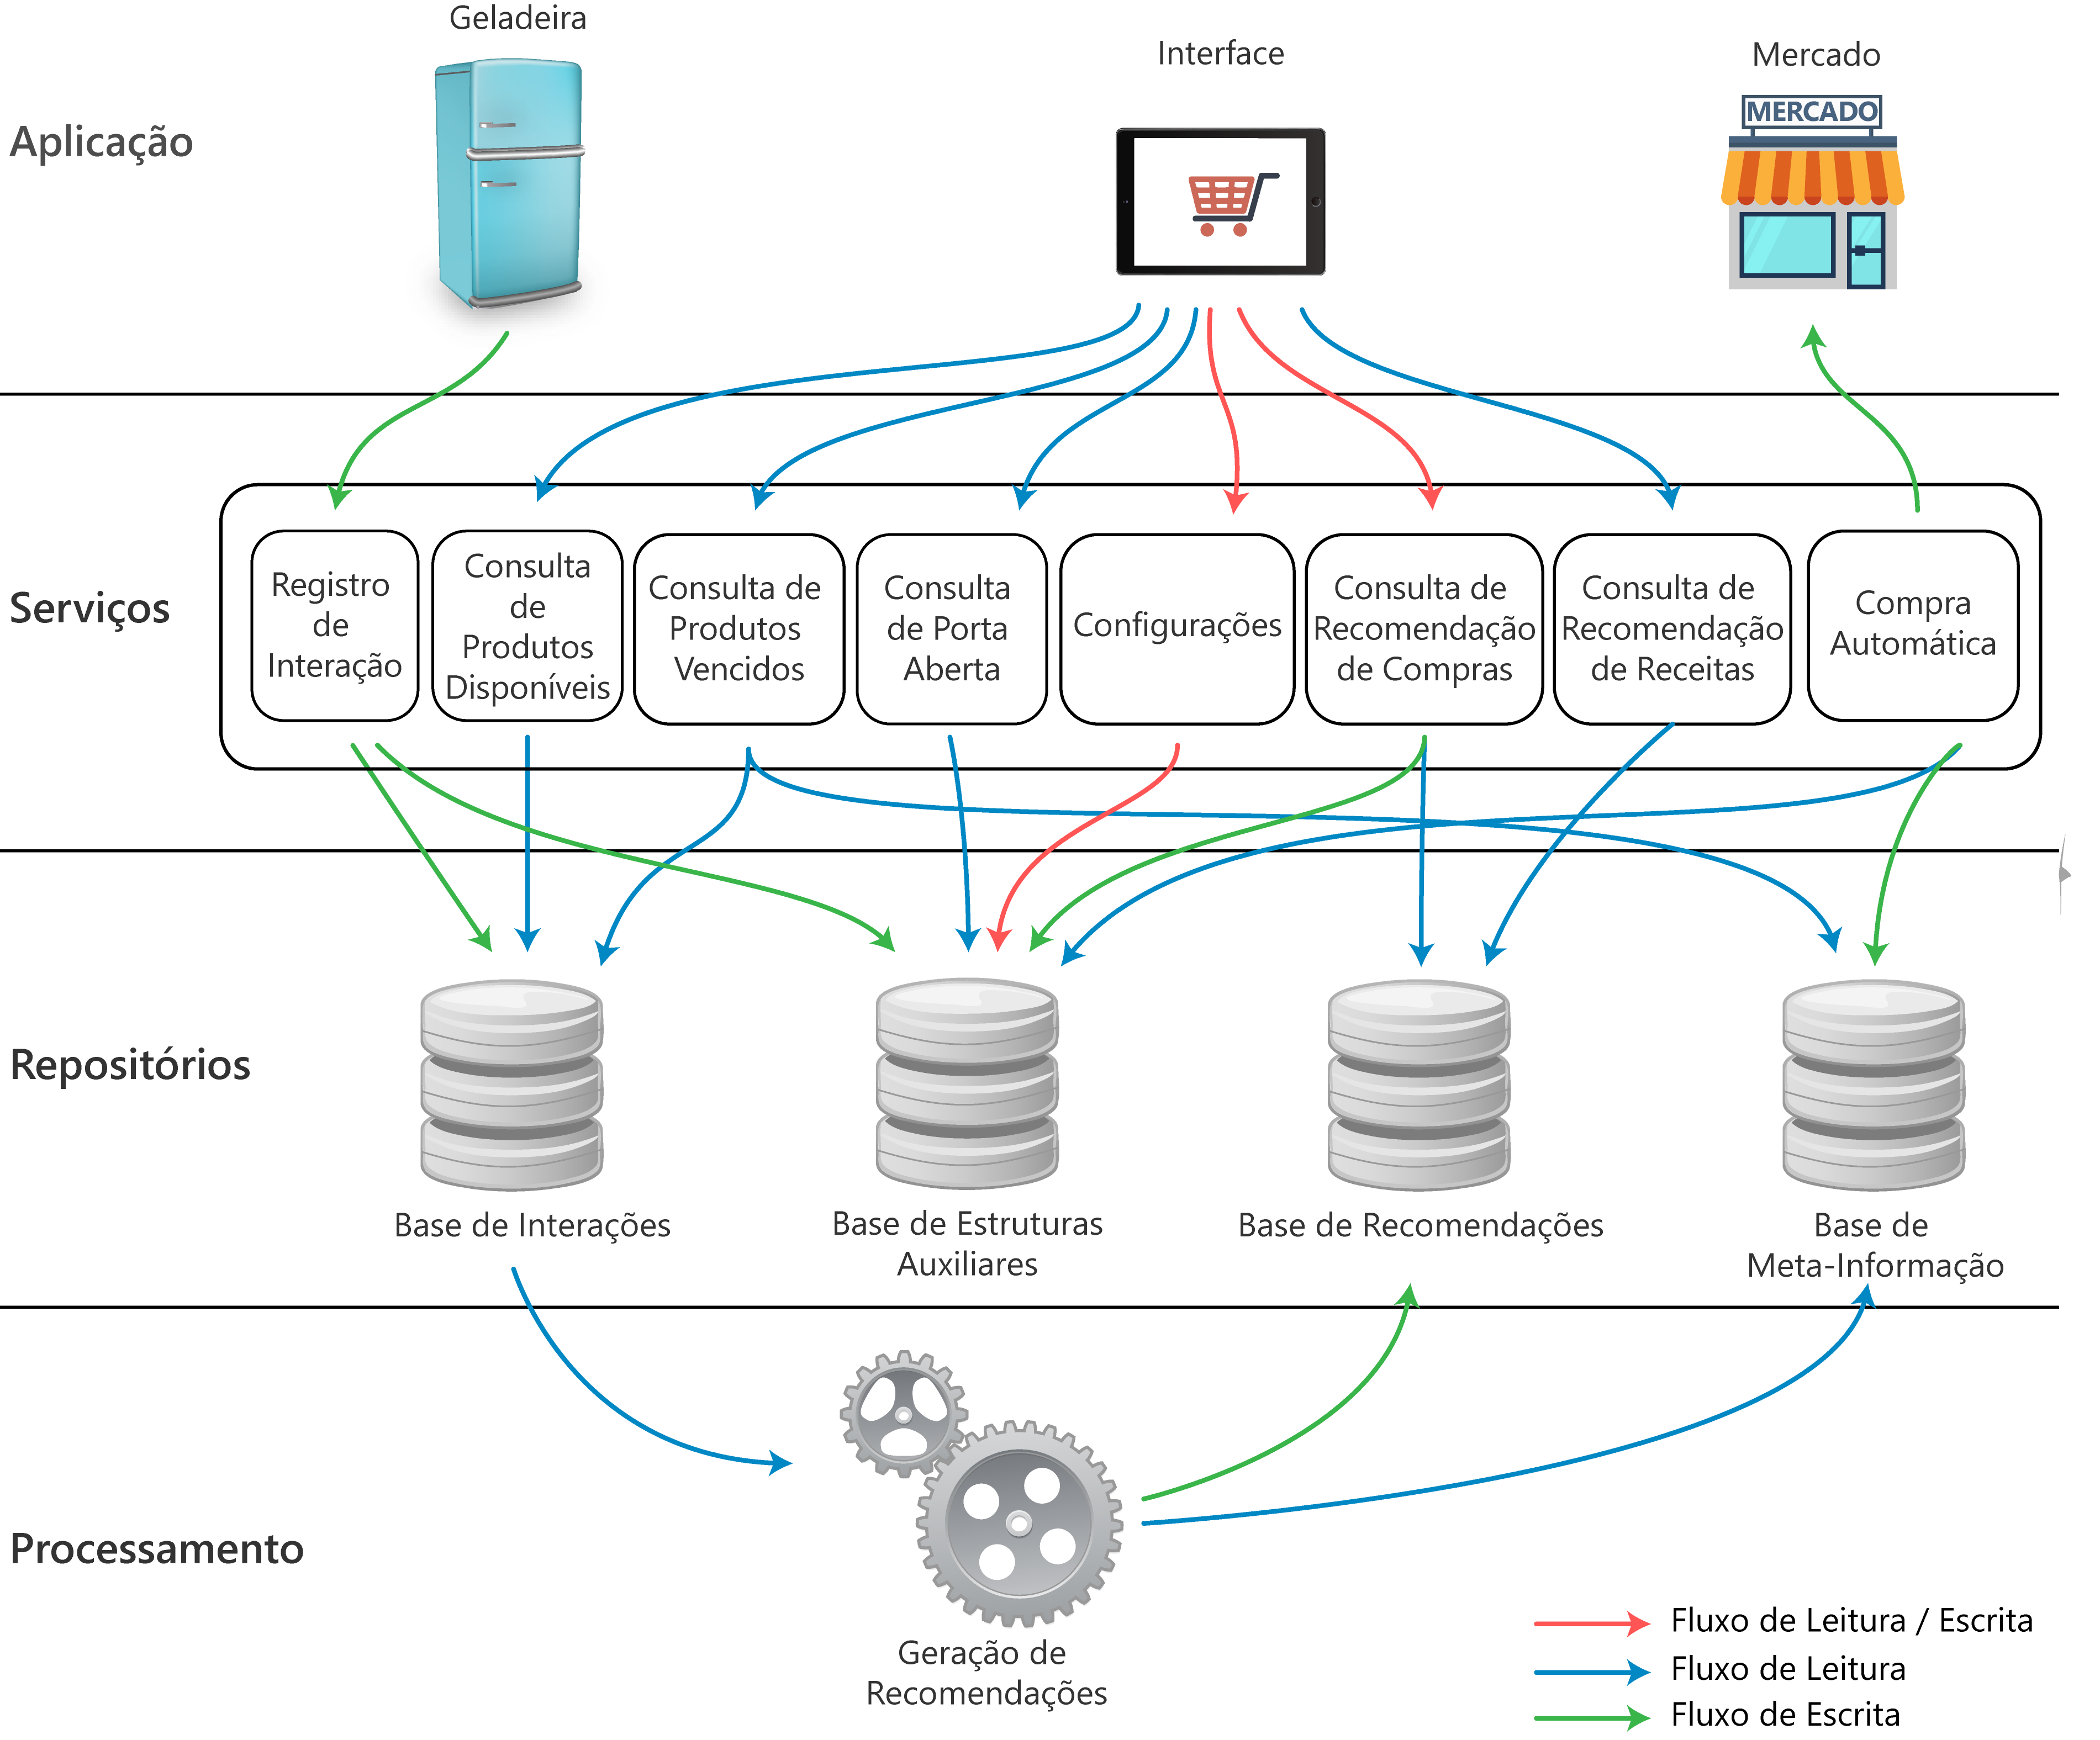
\includegraphics[width=0.92\textwidth]{modelo-logico}
    
    Fonte: Autores
\end{figure}
\nocite{Freepik2017} % fonte dos ícones

\subsection{Camada de Aplicação}

% Explanação sobre a camada

% Descrição da geladeira
%  - O que é
%  - Qual objetivo
%  - Porque

A camada de aplicação, como descrito, envolve os componentes  externos ao sistema principal. O primeiro deles é a geladeira à qual é responsável por monitorar os produtos nela contidos. Deste modo, a cada interação do usuário com a geladeira, é realizada uma varredura a fim de verificar o conjunto de produtos existentes. Em seguida, envia-se tais informações para o servidor através do serviço de registro de interação.

Outra funcionalidade à qual a geladeira também é incumbida, é a verificação da condição de fechamento porta e, caso aberta por um determinado período, a geladeira faz um registro na base de estruturas auxiliares através do serviço de registro de interação para que o sistema seja capaz de emitir um aviso ao usuário.

% Descrição da interface
%  - O que é
%  - Qual objetivo
%  - Porque

O componente seguinte é a interface de usuário, incorporada à porta da geladeira. Ela se responsabiliza por permitir ao usuário a interação com o eletrodoméstico. Assim, tem-se como funcionalidades deste componente: a listagem de produtos contidos, produtos com prazos de validade próximos, notificações de alerta caso o usuário esqueça a porta aberta, configurações personalizáveis e, por fim, recomendações de possíveis compras de produtos e receitas.

As recomendações podem ser exibidas automaticamente ou quando o usuário desejar. Assim a aplicação faz, automaticamente, a requisição e alerta o usuário através de uma notificação ou, ainda, o usuário solicita as recomendações através da interface.

% Descrição do mercado
%  - O que é
%  - Qual objetivo
%  - Porque

%O último componente da camada de aplicação é o mercado. 
%A partir deste será possível fazer verificações da existência de produtos da geladeira com prazo de validade expirados. 
%Além disso, permite que, 


%  é possível fazer consultas de promoções de itens que eventualmente serão disponibilizadas pelo mercado.

\subsection{Camada de Serviços}

A camada de serviços disponibiliza um conjunto de funcionalidades aos componentes da camada de aplicação, se comportando como porta de entrada do sistema principal. Assim, há um conjunto de serviços específicos disponibilizados conforme a Figura \ref{fig:c4_modelo_logico} e que serão descritos nos parágrafos seguintes.

% Explanação sobre a camada serviços

% Descrição do "Registro de interação"
%  - O que é
%  - Qual objetivo
%  - Porque
O serviço de registro de interação receberá informações dos itens contidos da geladeira além do alerta de porta aberta. Em seguida, registra-se tais informações na base de interações e de estruturas auxiliares, respectivamente.


% Descrição do "Consulta de Produtos Disponíveis"
%  - O que é
%  - Qual objetivo
%  - Porque

Já o serviço de consulta de produtos disponíveis será requisitado pelo usuário através da interface. Então, será feita uma busca na base de interações pelo último registro feito ao qual conterá os produtos existentes no momento.

% Descrição do "Consulta de produtos vencidos"
%  - O que é
%  - Qual objetivo
%  - Porque

O serviço de consulta de produtos vencidos é acionado periodicamente pela interface. Desse modo, é feita uma busca pelo itens disponíveis na geladeira e o tempo que estão presentes, através da base de interações. Logo após, se faz uma consulta na base de meta-informação para determinar o período de validade (após aberto) de cada produto encontrado. A partir da comparação entre tempo de acondicionamento e prazo de expiração, sabe-se se o produto está vencido ou não. A estimativa é feita pois o prazo de validade transcrito em produtos não condiz após a abertura sua abertura. Assim, uma estimativa de tempo menor é necessária.

% Descrição do "Consulta de porta aberta"
%  - O que é
%  - Qual objetivo
%  - Porque
O serviço de consulta de porta aberta é requisitado pela interface de usuário periodicamente de forma automática. Como efeito da requisição, faz-se uma consulta à base de estruturas auxiliares a fim verificar a existência de um registro recente de porta aberta. O resultado é então encaminhado para a interface que alertará o usuário, caso necessário.

% TODO: O último registro diz se a porta está aberta ou não.

% Descrição do "Configurações"
%  - O que é
%  - Qual objetivo
%  - Porque

O serviço de configurações permite que o usuário personalize algumas características do funcionamento da geladeira. A primeira delas se refere ao mercado no qual as compras são realizadas. Além disso, é possível determinar quais produtos devem, sempre, estar disponíveis para consumo e qual a quantidade mínima necessária.

% Descrição do "Consulta de Recomendação de Compras"
%  - O que é
%  - Qual objetivo
%  - Porque

O serviço de consulta de recomendação de compras é requisitado pela aplicação periodicamente e também pelo usuário. Assim, quando é feita uma requisição, automática ou não, o serviço faz uma consulta à base de recomendações em busca de possíveis sugestões. O conjunto existente é então retornado para a interface que, por sua vez, indaga ao usuário se deseja realizar a compra e quais produtos deseja adquirir, dentre os apresentados. A lista é retornada ao serviço que, então, faz o registro na base de estruturas auxiliares.

% Descrição do "Consulta de Recomendação de Receitas"
%  - O que é
%  - Qual objetivo
%  - Porque

O serviço de recomendação de receitas recebe uma requisição do usuário e faz uma consulta à base de recomendações. Caso existam receitas para recomendar, essas serão listadas ao usuário na interface e será possível então a escolha de qual receita deseja-se visualizar.

% Descrição do "Compra automática"
%  - O que é
%  - Qual objetivo
%  - Porque

\subsection{Camada de Repositórios}\label{sec:camada-repo}

% Explanação sobre a camada
O conjunto de repositórios desta camada atuam na persistência de informações geradas pelos diversos componentes das camadas de aplicação e de processamento. Nessa modelagem, dividiu-se em quatro bases: de interações, de estruturas auxiliares, de recomendações e de meta-informação.
A primeira base é responsável, como descrito anteriormente, pelo registro de produtos acondicionados na geladeira. A partir disso, as consultas realizadas nessa base recuperarão os itens constantes após cada interação do usuário.

A base de estruturas auxiliares contém informações que são utilizadas por mais de um serviço. Tais informações são alertas de porta aberta, configurações e as listas de compras determinadas pelo usuário. 

Já a base de recomendações armazena todas as sugestões de receitas e de compras construídas pelo gerador e que serão apresentadas ao usuário.

A última base, de meta-informação contém informações referentes ao conteúdo dos produtos adquiridos e que são utilizadas pelo gerador de recomendações e pelo serviço de verificação de produtos vencidos. Tais informações incluem características do produto, como código de barras, fabricante, informações nutricionais, categoria além do tempo estimado de validade.

\subsection{Camada de Processamento}

% Explanação sobre a camada
A camada de processamento contém os módulos de geração de recomendações, de compras automáticas e de sincronização de meta-informação. O módulo de geração de recomendações faz uso das informações armazenadas na base de interação e das características de cada item mantidas na base de meta-informações.

% Como vai receber do mercado informações de que tem itens em promoção.
As recomendações de receitas fazem uso da base de interações para ter conhecimento dos produtos contidos atualmente e de meta-informações para resgatar as receitas e seus respectivos ingredientes. A partir disso, é feita uma comparação entre as bases. Caso alguma receita requeira itens que já estão presentes, essa será recomendada ao usuário. Do contrário, caso apenas alguns itens estejam em falta, será sugerida, ao usuário, além da receita, a compra dos produtos faltantes.

Compras são sugeridas com base na quantidade existente de um certo produto. Assim, quando tal valor cai abaixo da quantidade mínima, determinada pelo usuário, é feita a recomendação de compra do mesmo item. No entanto, o mercado pode não ter à disposição o produto específico, mas pode conter similares. Nesse caso, o sistema faz uma busca por itens similares e pede a aprovação do usuário para a compra deste, ao invés do original. Além disso, sugere-se novos itens com base em promoções de produtos, aos quais se tenha apresentado interesse, que, por ventura, o mercado venha a disponibilizar.

O processo de compra automática é executado automaticamente quando há uma lista de compras pendente. Assim, a partir da verificação de tal pendência na base de estruturas auxiliares, a compra é requisitada ao mercado. 

O processo de sincronização de meta-dados, periodicamente consulta o serviço de sincronização do mercado para verificar se há meta-informações de produtos às quais foram adicionados ou 
alterados.

\subsection{Camada de Agente Externo}

O componente desta camada é o mercado. Através dele, será possível verificar disponibilidade de produtos e efetivar as compras a partir da lista de produtos selecionados pelo usuário. Além disso, há a funcionalidade de sincronização de meta-informação de produtos onde, para isso, o mercado disponibiliza um serviço possibilitando, assim, que a base de meta-informação possa ser periodicamente atualizada. Essas informações serão utilizadas posteriormente na recomendação de produtos e receitas.


\section{Modelo físico}
% Descrição da geladeira
%  - O que é
%  - Qual objetivo
%  - Porque

% Explicar o que há dentro de cada componente lógico
% Se preciso desenhar a arquitetura interna do componente
% Por exemplo a geladeira, vai ter muitas coisas dentro que devem ser explicitadas

\begin{figure}[htb]
    \caption{Modelo físico}
    \label{fig:c4_modelo_fisico}
    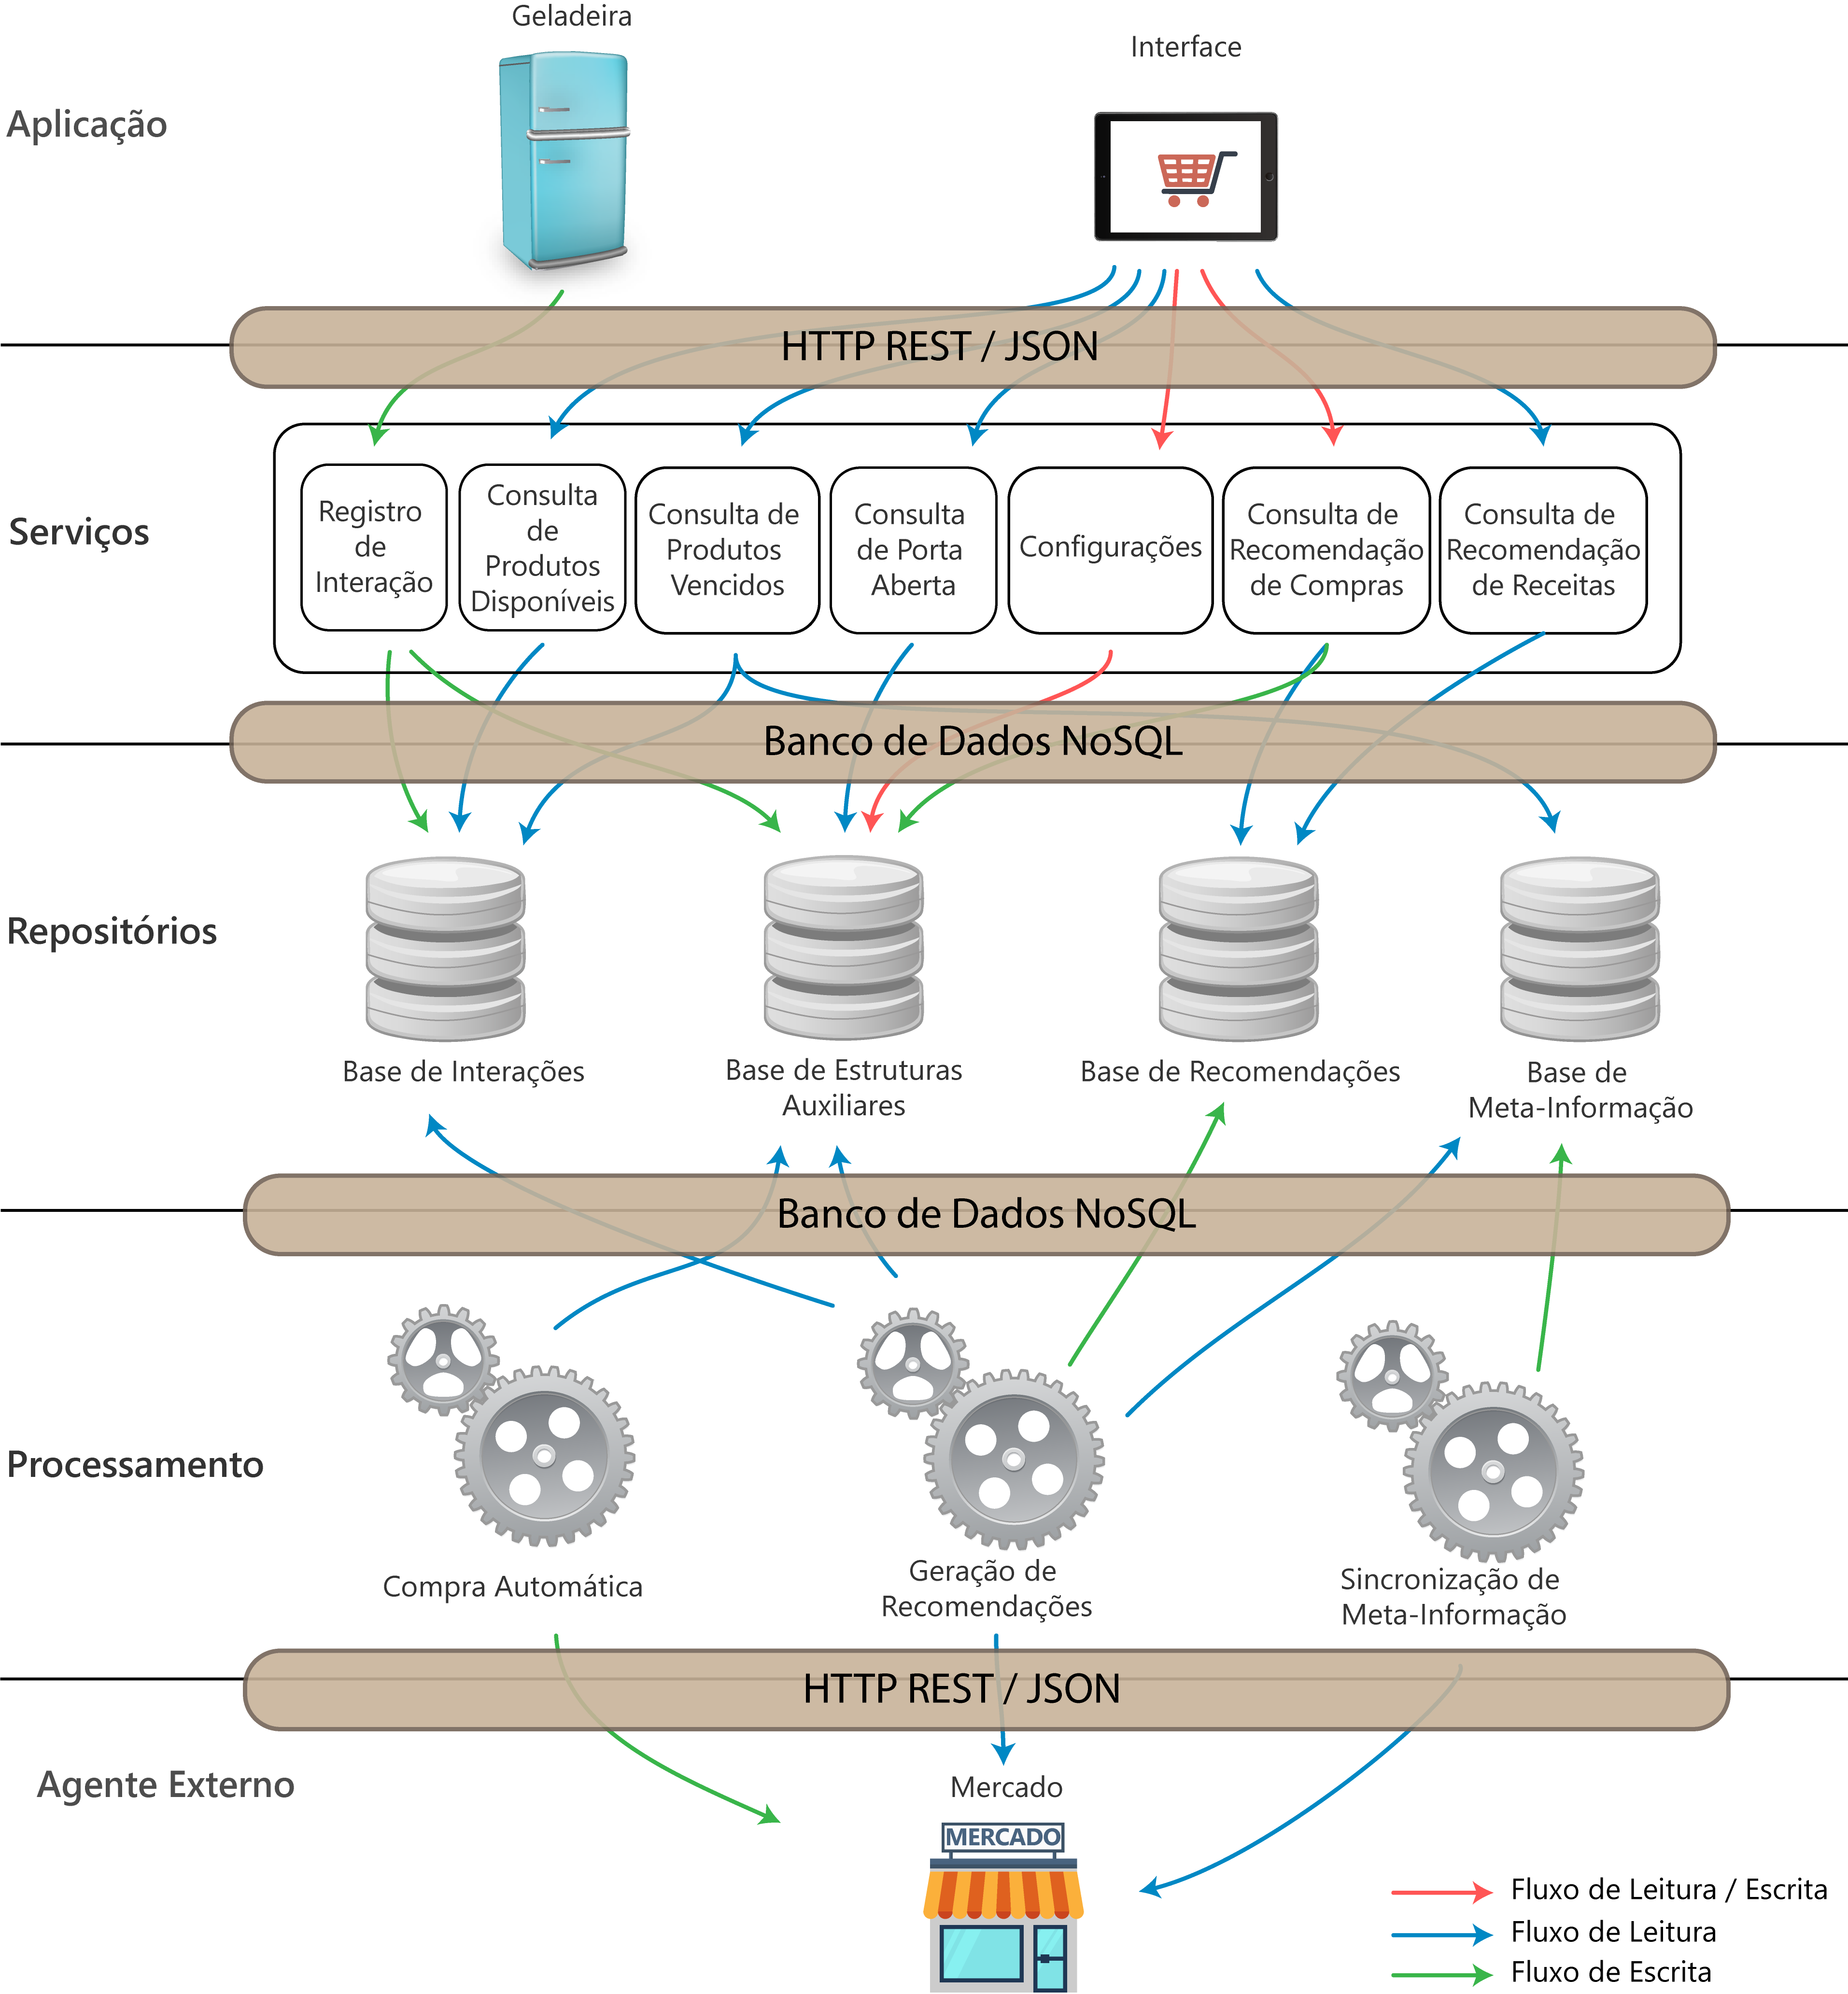
\includegraphics[width=0.8\textwidth]{c4_modelo-fisico.png}
\end{figure}

%%%%%%%%%%%%%%%%%%%%%%%%%%%%%%%%%%%%%%%%%%%%%%%%%%%%%%%%
\subsection{Camada de Aplicação}

\subsubsection{Geladeira}

A geladeira, presente no modelo lógido da Figura \ref{fig:c4_modelo_logico}, foi construída de acordo com a Figura \ref{fig:cap4_estr_geladeira}. Assim, observa-se três componentes principais: os leitores de etiquetas MFCR522 para RFID e NFC e o sensor de fechamento para a porta e a placa Raspberry PI\textsuperscript{\textregistered}\footnote{https://www.raspberrypi.org} 3 Modelo B. O primeiro deles, o conjunto de leitores, responsabiliza-se por efetuar leituras de possíveis etiquetas próximas a cada leitor quando for requerido. A partir disso, os dados lidos, referentes aos produtos, serão transferidos para o Raspberry PI que, por sua vez, os transfere para o serviço de Registro de Interação. Os dados das etiquetas se encontram no formato EPC, no qual, identifica-se o fabricante, a classe, o produto e a instância do produto a partir de um número de 96 bits, de forma semelhante ao código de barras presente nos produtos.

O sensor de fechamento de porta, por outro lado, é responsável por determinar quando ações devem ocorrer. O seu funcionamento envolve dois componentes: o primeiro é dotado de um imã e o outro contém um mecanismo que é influenciado pela presença ou não do ímã. Assim, quando estes se aproximam, indicando fechamento da porta, haverá um curto-circuito entre os terminais do mecanismo. Já quando afastados, indica-se abertura existindo, então, tem-se um circuito aberto.

Considerando-se, primeiramente, o evento de abertura da porta. Caso o usuário não a feche durante um determinado período de tempo, será feita uma requisição, através da placa Raspberry PI, para o serviço de registro de interação, indicando a situação. No entanto, no caso oposto, ou seja, quando ocorrer o fechamento da porta, dentro do período estipulado, realiza-se uma varredura dos produtos e, em seguida, uma requisição é enviada ao serviço para o registro de interação com o usuário.

Por fim, o último componente, o Raspberry PI, opera como um centro de controle, onde obtém dados do sensor de fechamento para, então, comandar leituras de etiquetas e/ou fazer requisições descritas anteriormente.

Para a comunicação entre os três componentes fez-se uso de dois protocolos específicos: a Interface Periférica Serial (SPI) e Protocolo de Transferência de Hipertexto (HTTP) com Transferência de Estado Representacional (REST). O primeiro deles foi empregado na comunicação entre os leitores RFID e o Rasbpberry, já o segundo, para troca de informações entre o Raspberry e o serviço de registro. Por fim, a comunicação com o sensor de fechamento se deu através de sinais digitais.

% FALAR SOBRE O PROTOCOLO USADO EM CADA PONTO

\begin{figure}[htb]
    \caption{Estrutura interna da geladeira}
    \label{fig:cap4_estr_geladeira}
    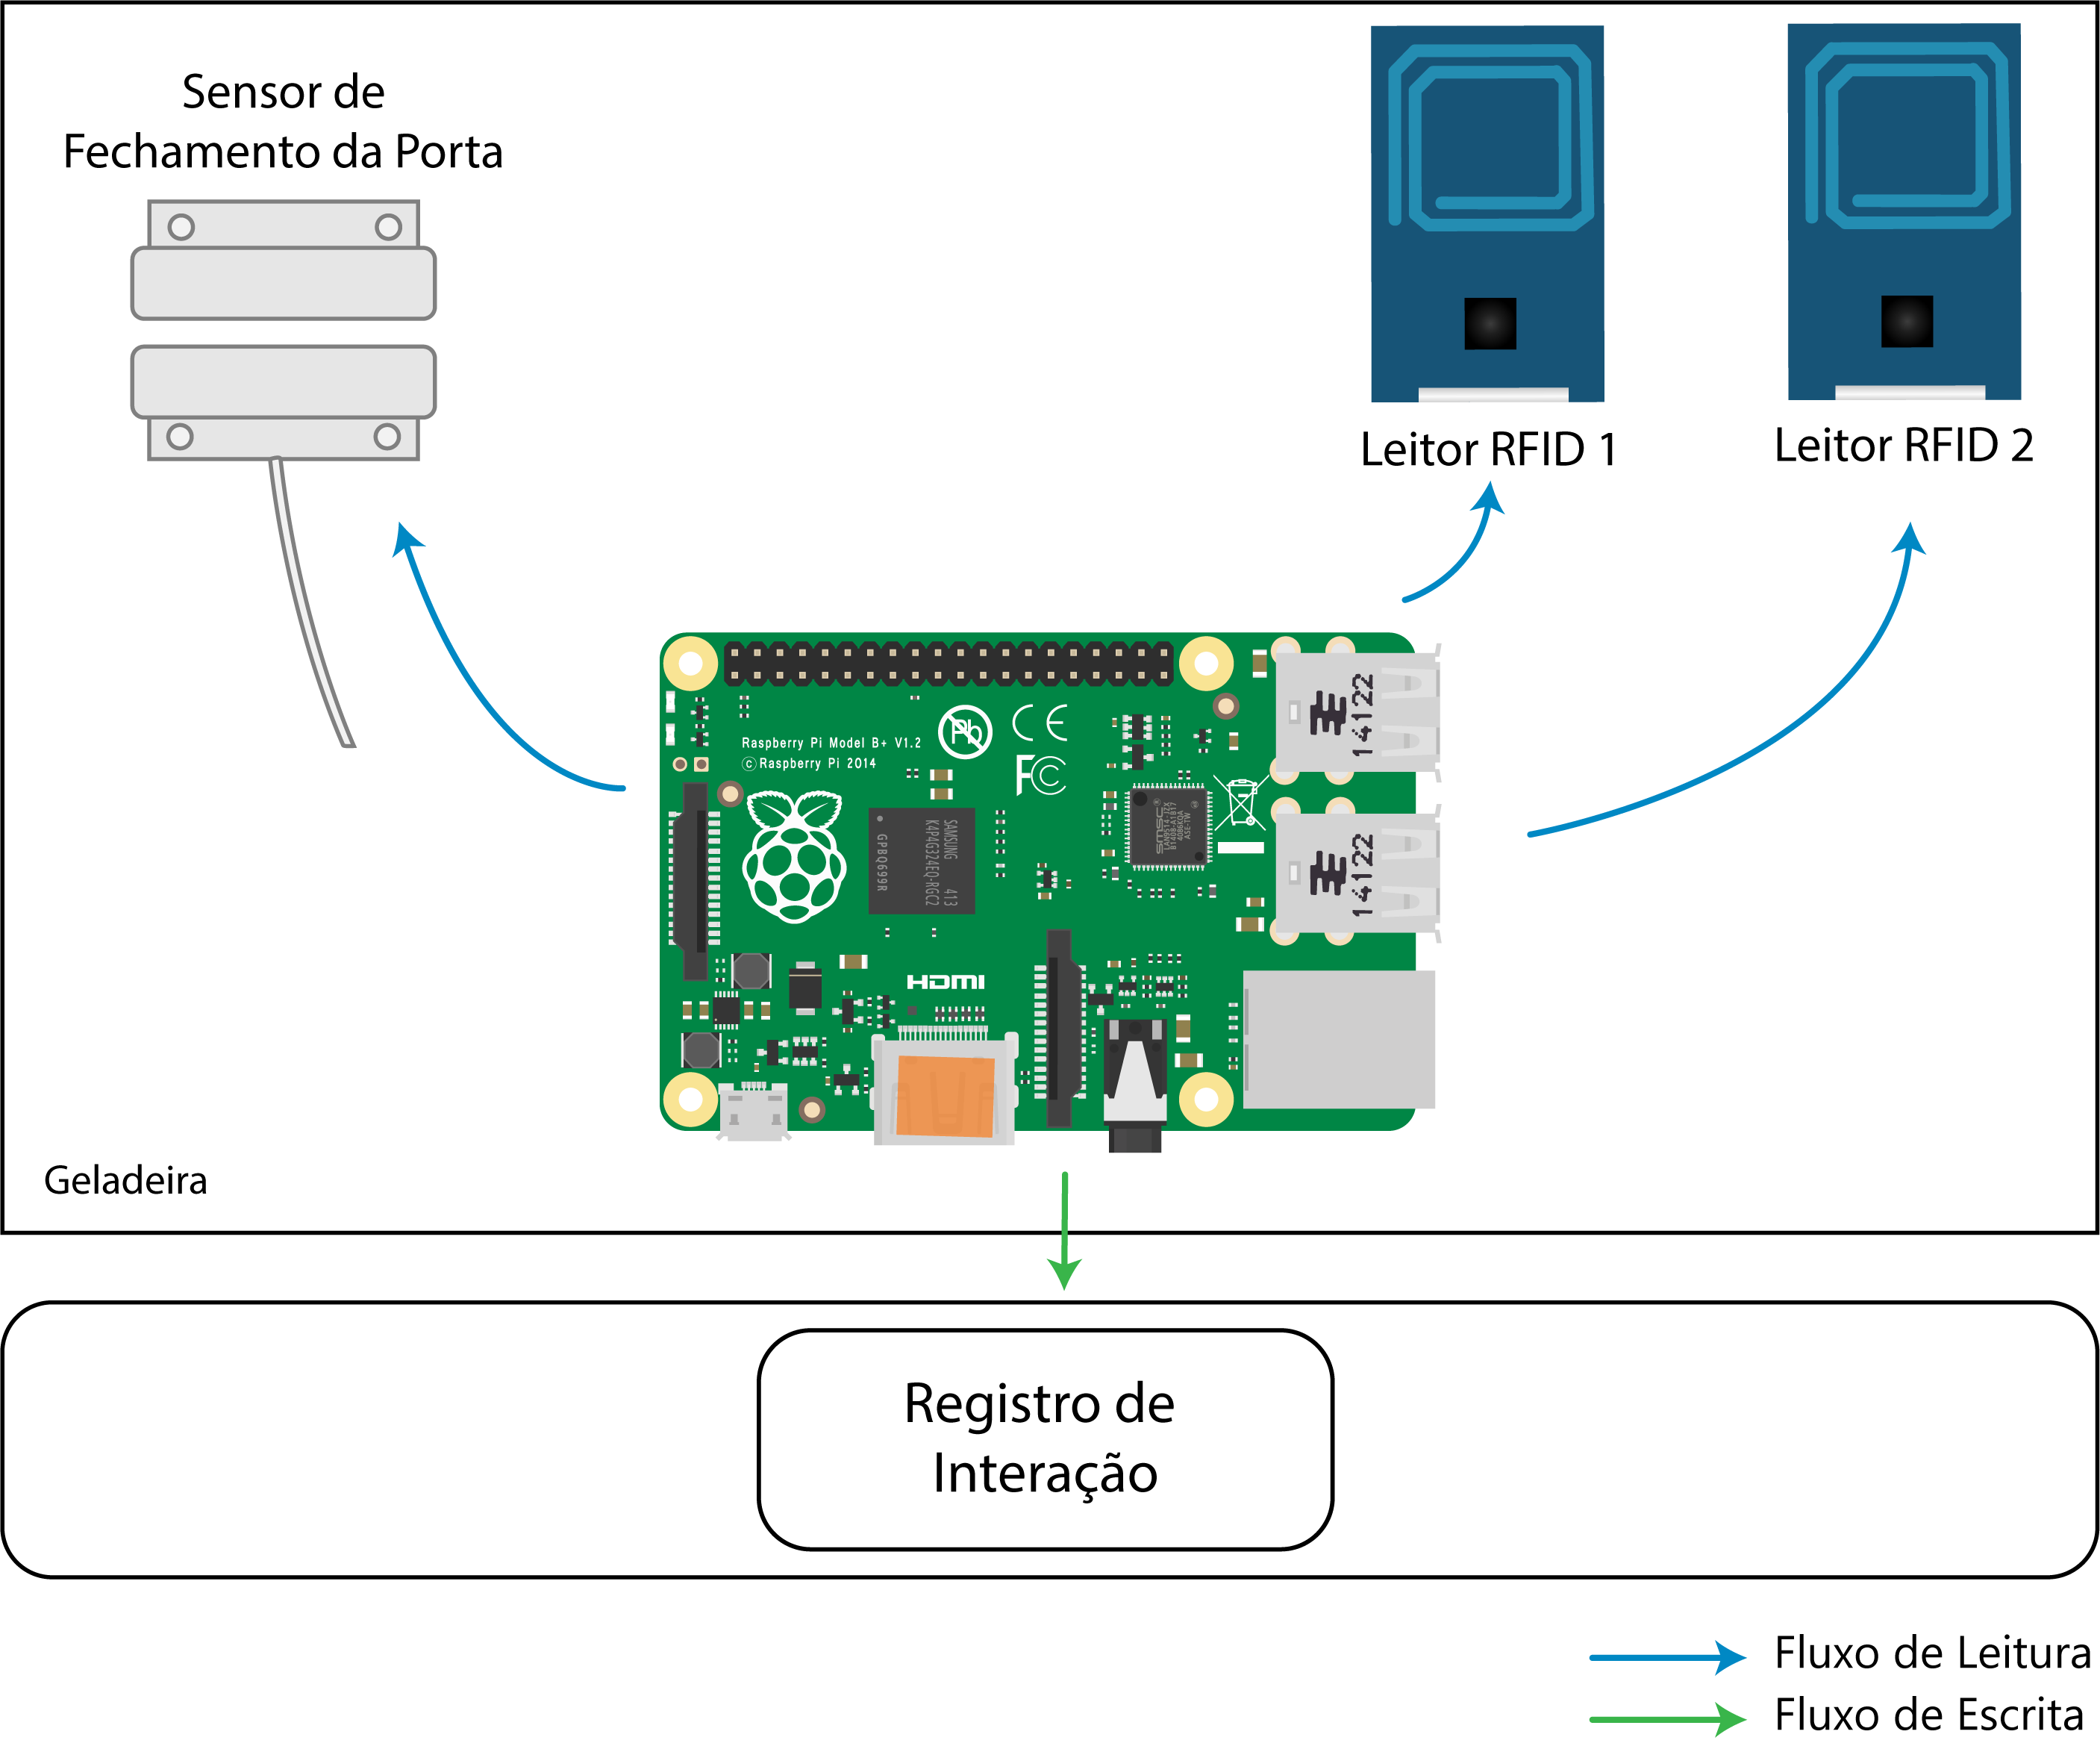
\includegraphics[width=\textwidth]{figuras/c4_modelo-logico-hardware.png}
    
    Fonte: Autores
\end{figure}
% Colocar a imagem

% Explicar cada componente

\subsubsection{Interface de Usuário}

\subsubsection{Mecanismo de Geração de Recomendações (\textit{Rascunho})}

Para a geração de recomendações de compras de produtos, tem-se duas situações: de acordo com os produtos que acabaram e de acordo com o que pode gostar. No primeiro caso, utiliza-se um híbrido entre filtragem colaborativa e baseada em conteúdo. Assim, será verificada a ausência de produtos que o usuário acha importante e a compra dos respectivos produtos será recomendada. Caso o produto em específico não esteja disponível, será avaliada a disponibilidade de produtos semelhantes e que outros usuários com gostos semelhantes também compraram e estes serão sugeridos. Já no segundo caso, será feito uma simples filtragem colaborativa onde, eventualmente, serão sugeridos produtos de acordo com os gostos do usuário em comparação com os demais.

Para a geração de recomendações de receitas, tem-se duas situações: de acordo com o que tem disponível e de acordo com o que gosta. No primeiro caso, será feito uma busca por receitas que podem ser preparadas com os produtos contidos na geladeira a partir de abordagem baseada em conteúdo. Já a segunda, será feita a partir dos gostos do usuário considerando os dos outros e o conteúdo dos itens que mais gosta, ou seja, as receitas devem conter os produtos que o usuário mais gosta.

%%%%%%%%%%%%%%%%%%%%%%%%%%%%%%%%%%%%%%%%%%%%%%%%%%%%%%%%
\subsection{Camada de Serviços}
\lipsum[1]

\subsubsection{Registro de Interação}

\subsubsection{Consulta de Produtos Disponíveis}

\subsubsection{Consulta de Produtos Vencidos}

\subsubsection{Consulta de Porta Aberta}

\subsubsection{Configurações}

\subsubsection{Consulta de Recomendações de Compras}

\subsubsection{Consulta de Recomendações de Receitas}


%%%%%%%%%%%%%%%%%%%%%%%%%%%%%%%%%%%%%%%%%%%%%%%%%%%%%%%%
\subsection{Camada de Repositórios}

As bases de dados nesse trabalho estão relacionadas ao servidor principal de serviços e recomendação. Conforme a Figura \ref{fig:c4_modelo_fisico} e, como já dito, tem-se quatro bases de dados: de interações, estruturas auxiliares, recomendações e metainformação. Tais bases dão suporte para todas as funcionalidades do sistema, desde registro de interação até resgate de metainformações de produtos. 

A tecnologia utilizada para implementação dos repositórios baseia-se no conceito de banco de dados não relacionais, como o NoSQL. Tem-se como principal característica, nesse conceito, o não-suporte ao SQL (Search Query Language) para alcance de performance ou confiabilidade. O intuito desse tipo de banco de dados é ser utilizado em aplicações de grande escala, nas quais supera o desempenho de bancos relacionais. Os dados são registrados em coleções, que não restringem os tipos de dados armazenáveis. Consequentemente, é possível, por exemplo, registrar, em uma mesma coleção, cadastros de usuários e de fornecedores. \cite{Boicea2012}. 

Neste trabalho, optou-se pelo MongoDB\textsuperscript{\textregistered}, um sistema de banco de dados NoSQL baseado em documentos, ao qual o armazenamento decorre no formato JSON, um formato baseado em chave e valor. 

O sistema deste trabalho apresenta o comportamento de interações constantes com as bases de dados, provenientes de diversos dispositivos, seja na forma de inserções como resgates de informação. Por isso, na implementação utilizou-se o conceito de base de dados NoSQL.

Nas seções que seguem, os repositórios serão detalhados em seus aspectos internos, como tipos de dados armazenadas, a origem da necessidade destes e em que momento são utilizados.

\subsubsection{Base de Interações}

Como descrito na Seção \ref{sec:camada-repo}, essa camada é responsável pelo registro das interações de usuários com produtos. A cada registro, ter-se-á um conjunto de códigos EPC de itens atuais, além da identificação da geladeira e o \textit{timestamp}, ou seja, o momento no qual ocorreu a interação. A Figura \ref{fig:cap4_base-int_json}, demonstra um registro tal qual como é inserido na base.

\begin{figure}[htb]
    \caption{Registro na base de interações}
    \label{fig:cap4_base-int_json}
    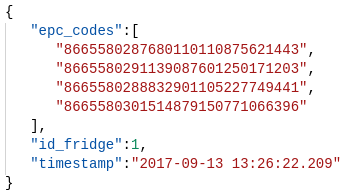
\includegraphics[width=0.45\textwidth]{cap4_base-int_json}
    
    Fonte: Autor
\end{figure}

Nota-se, pela Figura \ref{fig:cap4_base-int_json}, que havia quatro itens na geladeira no dia 13 de setembro de 2017 à 13h26. No entanto, não é claro quais produtos estão contidos. Para tanto, operações de deslocamento de bit são realizadas sobre o código EPC revelando, desse modo, o fabricante, o produto e o número de série da instância. A Figura \ref{fig:cap4_epc} exibe estrutura de um código EPC.

\begin{figure}[htb]
    \caption{Estrutura de um código EPC}
    \label{fig:cap4_epc}
    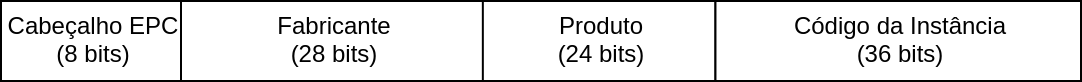
\includegraphics[width=\textwidth]{cap4_epc}
    
    Fonte: Autor
\end{figure}

Esse tipo de registro é a principal fonte de informação a cerca dos hábitos dos usuários, uma vez que explicita os produtos com os quais o usuários mais têm contato, bem como os horários em que isso ocorre. A partir dessas informações, é possível calcular as recomendações.


\subsubsection{Base de Estruturas Auxiliares}

A base de estruturas auxiliares tem como principal objetivo intermediar a comunicação entre serviços e entre processos. Assim, ela contém diversos tipos de registros, sendo eles, de estado da porta, configurações de cada geladeira e listas de compras pendentes.

O primeiro dos registros, informa qual o último estado registrado por uma determinada geladeira, ou seja, aberto ou fechado. Assim, tal informação será requisitada pela interface, através do registro de consulta de porta, e alertará o usuário caso necessário. A Figura \ref{fig:cap4_aux_setting}, demonstra um registro de estado da porta.

\begin{figure}[htb]
    \caption{Estrutura de um registro de estado da porta}
    \label{fig:cap4_aux_setting}
    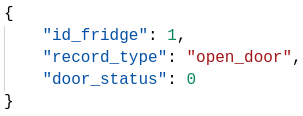
\includegraphics[width=0.35\textwidth]{cap4_aux_setting}
    
    Fonte: Autor
\end{figure}

Como é visível na Figura \ref{fig:cap4_aux_setting}, três informações são guardadas: a identificação da geladeira, o tipo de registro que será inserido, ou seja, estado da porta, e o estado em si. Segundo a implementação, ``0'' significa porta aberta e, ``1'', fechada.

O segundo tipo de registro, de configurações, mantém um conjunto de parâmetros específicos de cada geladeira. Esses parâmetros se referem serviço do mercado no qual às compras são realizadas e metainformações de produtos e receitas são resgatadas; ao tempo para que a porta da geladeira deve permanecer aberta antes que a interface notifique o usuário; ao período mínimo entre compras automáticas e os produtos que o usuário deseja que estejam sempre disponíveis. As demais informações se referem à identificação da geladeira bem como o tipo de registro, nesse caso, de configurações.

As informações referentes ao mercado são utilizadas pelos processos do sistema, ou seja, de compra automática, recomendação e sincronização de meta-informação. Já informações de tempo de notificação são requisitados pela interface através do serviço de configurações. Por outro lado, o tempo mínimo entre compras é requisitado pelo processo de compras automáticas. Por fim, a lista de produtos requeridos pelo usuário é utilizada pelo processo de recomendação na sugestão de novas compras.

\begin{figure}[htb]
    \caption{Estrutura de um registro de configurações}
    \label{fig:cap4_settings}
    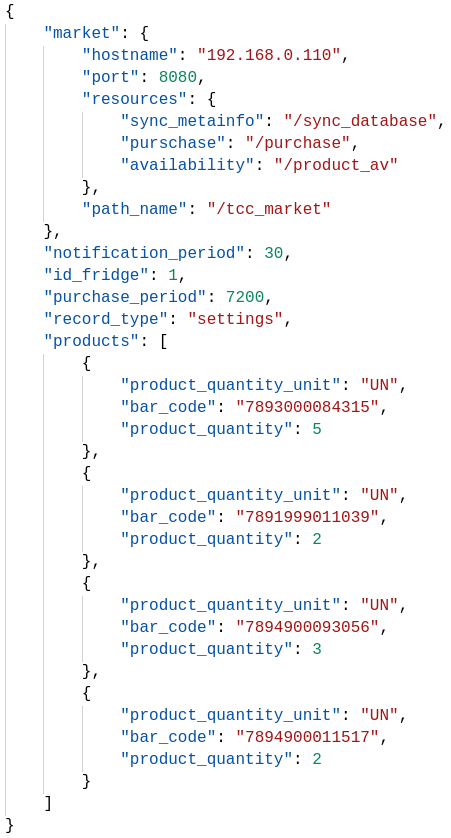
\includegraphics[width=0.5\textwidth]{cap4_settings}
    
    Fonte: Autor
\end{figure}

\subsubsection{Base de Recomendações}
abc


\subsubsection{Base de Meta-Informação}
abc

\begin{figure}[htb]
    \caption{Estrutura de um registro de metainformação de produto}
    \label{fig:cap4_metainfo}
    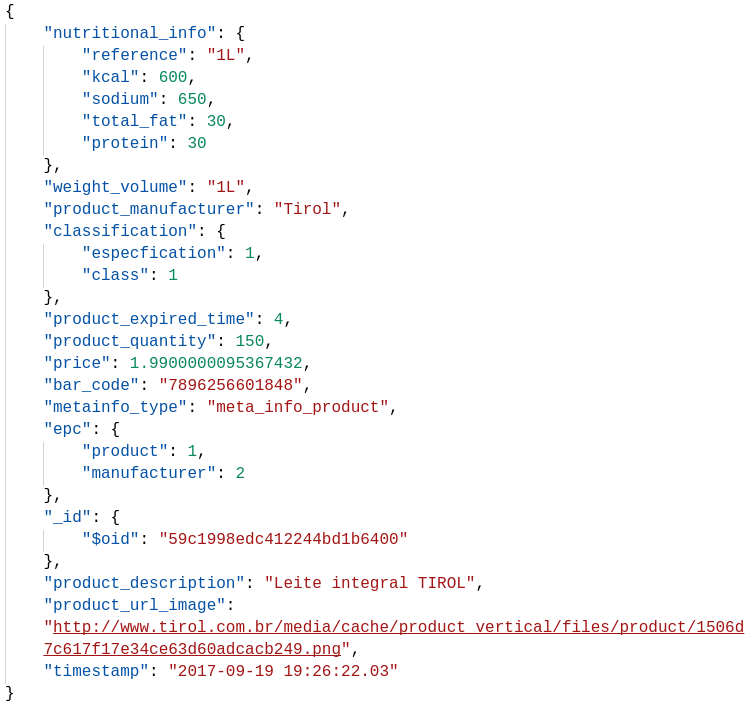
\includegraphics[width=\textwidth]{cap4_metainfo}
    
    Fonte: Autor
\end{figure}

%%%%%%%%%%%%%%%%%%%%%%%%%%%%%%%%%%%%%%%%%%%%%%%%%%%%%%%%

\subsection{Camada de Processamento}
\lipsum[1]
\subsubsection{Processo de Compras Automáticas}

\subsubsection{Processo de Geração de Recomendações}

\subsubsection{Processo de Sincronização de Meta-Informação}


%%%%%%%%%%%%%%%%%%%%%%%%%%%%%%%%%%%%%%%%%%%%%%%%%%%%%%%%
\subsection{Camada de Agente Externo}
\lipsum[1]

%#######################################################
\section{Exemplo de fluxo de execução}